\documentclass[french]{book}
\usepackage[utf8x]{inputenc}
\usepackage[T1]{fontenc}
\usepackage{babel}
\usepackage{lmodern}
\usepackage[top=2cm,bottom=2cm,left=3cm,right=3cm]{geometry}
\usepackage{microtype}
\usepackage{mathtools, amssymb, amsthm}
\usepackage{mdframed}
\usepackage{hyperref}
\usepackage{graphicx}
\usepackage{xcolor}
\usepackage{mathrsfs}
\usepackage{wrapfig}
\usepackage{stmaryrd}
\usepackage{framed}
\usepackage[Glenn]{fncychap}

\newtheorem{prototheorem}{Théorème}[section]
\newenvironment{thm}
   {\colorlet{shadecolor}{orange!10}\begin{shaded}\begin{prototheorem}}
   {\end{prototheorem}\end{shaded}}

\newtheorem*{protocorollary}{Corollaire}
\newenvironment{corollary}
    {\colorlet{shadecolor}{violet!10}\begin{shaded}\begin{protocorollary}}
    {\end{protocorollary}\end{shaded}}

\newtheorem*{protolemma}{Lemme}
\newenvironment{lemma}
    {\colorlet{shadecolor}{pink!15}\begin{shaded}\begin{protolemma}}
    {\end{protolemma}\end{shaded}}

\theoremstyle{definition}
\newtheorem{protodefinition}{Définition}[section]
\newenvironment{definition}
    {\colorlet{shadecolor}{green!5}\begin{shaded}\begin{protodefinition}}
    {\end{protodefinition}\end{shaded}}

\newtheorem{protoproposition}{Proposition}[section]
\newenvironment{prop}
    {\colorlet{shadecolor}{blue!5}\begin{shaded}\begin{protoproposition}}
    {\end{protoproposition}\end{shaded}}

\theoremstyle{remark}
\newtheorem*{remark}{Remarque}
\newtheorem{exo}{Exercice}
\newtheorem*{protoexemple}{Exemple}
\newenvironment{exemple}
    {\colorlet{shadecolor}{gray!10}\begin{shaded}\begin{protoexemple}}
    {\end{protoexemple}\end{shaded}}


\newcommand{\lesss}{<}
\newcommand{\less}{\lesss}

\newcommand{\biggg}{>}
\newcommand{\bg}{\biggg}

\title{\bsc{Analyse fonctionnelle et distributions}}
\date{2023-2024}

\begin{document}

\maketitle

\tableofcontents

\chapter{Espaces localement convexes}

\section{Rappels de topologie}

J. Dieudonné 1 et 2.

Reed-Simon 1, 2 et 4.

Brézis, ``Analyse fonctionnelle''

\

Soit $X$ ensemble. Soit $(X, \mathscr{T} )$ espace topologique où $\mathscr{T}  \subset \mathscr{P}(X) $.

$\mathscr{T} $ parcourt l'ensemble des voisinages de $x$ où $x$ est un point quelconque de $X$.

\subsection{Axiomes}

\begin{enumerate}
  \item Soient $x \in X$ et $ V'$ voisinage de $x$. Si $V \supset V'$ alors $V$ est un voisinage de $X$.
  \item $\bigcap_{\text{ finie } }  V_i$ est un voisinage de $x$, $\bigcap_{\text{ finie } } V_i \in \mathscr{T}  $,  mais $\bigcap_{\varepsilon \bg 0} V _{\varepsilon }  \neq \emptyset$ n'est pas un voisinage de $0$.
  \item $\bigcap_{i \in I} V_i $ est un voisinage de $x$.
\end{enumerate}


\begin{definition}[Ouvert]
  $\Omega$ ouvert si et seulement si $\Omega$ est voisinage de chacun de ses points.
\end{definition}


\begin{exemple}
  $(-1, 1)$ ouvert tandis que $[-1, 1)$ non ouvert car -1 n'a pas de voisinage.
\end{exemple}

\

$V(x) =(x- \varepsilon , x+ \varepsilon )$ est une base de voisinage pour la topologie usuelle de $\mathbb{R}$.

\begin{exo}
  On peut définir axiomatiquement $\mathscr{T} $ à partir de ses ouverts.
\end{exo}

\begin{definition}[Fermé]
  On dit que $F$ est un fermé si et seulement si $F ^{C}$ est un ouvert.
\end{definition}

\subsection{Cas particulier d'espaces topologiques : espaces métriques}



\begin{definition}[Espace métrique, distance] \label{distance}
  \

  $X$ est un ensemble, $d : X \times X \to \mathbb{R} ^{+}$ distance sur $X$ si et seulement si :
  \begin{enumerate}
    \item $d(x, y) = 0$ si et seulement si $x = y$ ;
    \begin{remark}
      Si on a seulement $x =y \implies d(x,y) =0$, alors $d$ est un écart.
    \end{remark}
    \item $d(x,y) = d(y,x)$ (symétrie) ;
    \item $d(x,y) \leq d(x,z) + d(z,y)$ (inégalité triangulaire).
    De ce fait, $\lvert d(x,z) - d(y,z) \rvert \leq d(x,y)$.
  \end{enumerate}
\end{definition}



\begin{exemple}
  \begin{enumerate}
    \item Dans $\mathbb{R}^n$, $d(x,y) = \Vert x-y \Vert $.
    \item $X$ ensemble. On définit $d$ de la façon suivante :
    $$ \forall x, y \in X,  d(x, y) = \begin{cases}
      d(x,y) =0 \text{ si } x=y \\
      d(x,y) = 1 \text{ si } x \neq y.
    \end{cases}$$

    Il s'agit de la distance triviale.

    Si $x,y,z$ distincts alors $d(x,y) \leq d(x,z)+d(z,y)$.
  \end{enumerate}

\end{exemple}


\subsection{Comparaison des topologies}

\

Soient $X$ un ensemble et $\mathscr{T}, \mathscr{T}' $ des topologies sur $X$.

\begin{definition}[Plus fine]
  On dit que $\mathscr{T}' $ est plus fine que $\mathscr{T} $ et on note $\mathscr{T}' \prec \mathscr{T}  $ si et seulement si $\mathscr{T} \subset \mathscr{T}' $.

  On dit aussi que $\mathscr{T}' $ est plus forte que $\mathscr{T} $.
\end{definition}

\begin{remark}
  Si $\mathscr{T}' \prec \mathscr{T}  $, il y a plus d'ouverts dans $\mathscr{T}' $ que dans $\mathscr{T} $ (idem pour les fermés).
\end{remark}

\begin{proof}
  Soit $\Omega$ ouvert dans $X$. On a $\Omega \in \mathscr{T}  \implies \Omega \in \mathscr{T}' $.

  Soit $F$ un fermé dans $X$. On a $F \in \mathscr{T}$, mais $ \Omega = F ^{C} \in \mathscr{T} \implies F ^{C} \in \mathscr{T}' $, donc $F \in \mathscr{T}' $.
\end{proof}

\paragraph{Formulations équivalentes}

\begin{enumerate}
  \item On suppose que $\mathscr{T}' \prec \mathscr{T} $. Si $\forall x \in X $, $U$ est un voisinage de  $x$ pour $\mathscr{T} $, alors $U $ voisinage de $x$ pour $\mathscr{T}' $, car si $U $ est un ouvert de $\mathscr{T} $, alors $U $ est un ouvert de $ \mathscr{T}' $.
  \item Pour l'application identité définie comme suit

  $$ id : (X, \mathscr{T}' ) \longrightarrow (X, \mathscr{T} ), $$

  %allant de $(X, \mathscr{T}')$ vers $(X, \mathscr{T} )$,

  on a $\mathscr{T}' \prec \mathscr{T}  $ si et seulement si $id $ est continue.
\end{enumerate}

\

Par exemple, prenons $X = \{ f :[0, 1] \to \mathbb{R} \} $. On prend $\mathscr{T} $ topologie de la convergence simple, i. e.

$f_n $ converge vers $ f$ simplement si $\forall x \in [0, 1], f_n(x) \to f(x)$.

\subparagraph{Ouverts de $\Omega$}

$$\Omega _{a, \varepsilon } = \{ f \in X \mid \sup _{i =1, \dots, k} \lvert f(a_i) \rvert \less \varepsilon \}, $$ avec $a = a_0, \dots, a_k \in [0, 1]$ et $\varepsilon  \bg 0$.

$\Omega _{a, \varepsilon } $ est un voisinage de 0 (la fonction nulle) dans $X$.

Pour $f_0 \in X$, $\Omega _{a, \varepsilon } + f_0$ est une base de voisinage de $f_0$, car $X$ est un espace vectoriel (on agit par translation).

\

On considère maintenant la topologie de la convergence uniforme $\mathscr{T}' $.

$\Omega _{\varepsilon } = \{ f \in X, \sup_{ x \in [0, 1] } \lvert f(x) \rvert \less \varepsilon   \} $ est un voisinage de $0$ (la fonction nulle).

\begin{prop}
  $\mathscr{T}' $ est plus fine que $\mathscr{T} $, ie $\mathscr{T} \subset \mathscr{T}' $.
\end{prop}

\begin{proof}
  Soit $\Omega _{a, \varepsilon } \in \mathscr{T}  $.

%  $f \in \Omega _{a, \varepsilon }$, alors on a $\lvert f(a_i) \rvert \less \varepsilon $.

  Si $f \in \Omega _{\varepsilon }$, alors $$\forall x \in [0, 1], \lvert f(x) \rvert \less \varepsilon, $$ ce qui implique que $$ \forall i \in \{ 1, \dots, k \}, \lvert f(a_i) \rvert \less \varepsilon \ (\text{car c'est vrai pour tout } x). $$

   Donc $\Omega  _{\varepsilon } $ est un voisinage de 0 dans $\mathscr{T} $. On a ainsi démontré que $\mathscr{T}' $ est plus fine que $\mathscr{T} $.

  %Or $\Omega _{a, \varepsilon } \subset \Omega _{\varepsilon }$, donc $\Omega _{ \varepsilon }$ est un voisinage de $0$ pour la topologie $\mathscr{T} $.
\end{proof}

\

On considère l'espace des fonctions continues $\mathcal{C}^0$ avec la norme $$ \Vert f \Vert _{0} = \sup_{  } \lvert f(x) \rvert $$ et l'espace des fonctions de classe $\mathcal{C}^1$ $\mathcal{C}^1$ avec la norme $$\Vert f \Vert _{1} = \sup \lvert f(x) \rvert + \sup \lvert f'(x) \rvert.$$

La topologie sur $\mathcal{C}^1$ est plus fine que celle sur $\mathcal{C}^0$.

\begin{proof}
  On a pour tout $f$, $$\Vert f \Vert _{0} \leq \Vert f \Vert _{1} .$$

  Ainsi si $$\Vert f \Vert _{1} \less \varepsilon,   $$ alors $$\Vert f \Vert _{0} \less \varepsilon.  $$

  Par conséquent, $\{ f , \Vert f \Vert _{1 } \less \varepsilon  \} \subset \{ f, \Vert f \Vert _{0} \less \varepsilon   \} $.

  Donc $\mathscr{T}' \prec \mathscr{T}  $.

  On sait également que si $U$ est un voisinage de 0 pour $\mathscr{T} $, alors $U$ est un voisinage de 0 pour $\mathscr{T}' $.
\end{proof}

\paragraph{Topologie métrisable (exemples)}

\begin{enumerate}
  \item Topologie grossière $\mathscr{T}= \{ \emptyset, X \} $. C'est la topologie la moins fine.

  \begin{remark}
    $\mathscr{T}' = \mathscr{P}(X)  $ est la topologie la plus fine.
  \end{remark}

  Vérifions si la topologie grossière est métrisable dans différents cas.
  \begin{itemize}
    \item Si $X = \{ a \} $, on a $d(a,a) =0$. Le seul voisinage de $a$ est $X = \{ a \} $. Donc $\mathscr{T} $ est métrisable.
    \item Supposons que $X = \{ a,b \} $. Mais $\mathscr{T} $ n'est plus métrisable, avec $d(a,b) =1$ (distance triviale).

    Raisonnons par l'absurde. Si $\mathscr{T} $ était métrisable, $\mathscr{T} $ devrait contenir un ouvert $\Omega$ tel que $a \in \Omega$ et $b \notin \Omega$. Or $\mathscr{T} = \{ \emptyset, X \} $, donc c'est impossible.
  \end{itemize}

  Pour $\mathscr{T}' $, on choisit la distance $d$ telle que $d(x,y) = 0 \text{ ou } 1$. Est-ce que $\mathscr{T}' $ est métrisable ?

  \item Prenons $\mathscr{T} $ telle que $\mathscr{T} = \{ \emptyset, \{ a \} , X \} $.

  On suppose que $X$ contient au moins deux éléments. Dans ce cas, $\mathscr{T} $ est une topologie sur $X$ non métrisable, car si $d(a,b)=1,$ avec $ b \neq a$, alors dans $\mathscr{T} $ il n'existe pas de boule ouverte qui contient $\{ b \} $ sans contenir $\{ a \} $.

  \item Considérons $X = \{ a,b \}$ muni de la topologie $  \mathscr{T} = \{ \emptyset, \{ a \}, \{ b \}, X \} = \mathscr{P}(X)  $.

  On a $d(a,b) = 1$, car $a \neq b$.

  De ce fait :

  $\{ a \} $ voisinage de $a$ qui ne contient pas $b$ ( $\{ a \} = \{ x \text{ tel que } d(x,a) \less 1 \} $) ;

  $\{ b \} $ voisinage de $b$ qui ne contient pas $a$.




\end{enumerate}

\subsection{Espaces vectoriels topologiques}

Dans le cas où $(X, \mathscr{T} )$ est un espace vectoriel topologique, il suffit de connaître les voisinages de 0 et on agit par translation pour déterminer les voisinages de n'importe quel $x \in X$.

\begin{definition}[Continuité]
  Soient $X, Y$ deux espaces vectoriels topologiques et $f: X \to Y$ une application. On considère :

  \begin{gather*}
    (U_a) _{a \in A} \text{ voisinage de } 0 \text{ dans } X \\
    (V_b) _{b \in B} \text{ voisinage de } 0 \text{ dans  } Y
  \end{gather*}

  $f$ est continue si pour tout $V = V_b + f(x_0)$ dans $Y$, il existe $U = \bigcap_{\text{finie} } (U_a +x_0) $ voisinage de $x$ dans $X$ tel que $x \in U \implies f(x) \in V$.
\end{definition}

\paragraph{Cas particulier : $X$ normé}

\begin{definition}[Norme]
  $\Vert \cdot \Vert $ est une norme sur $X$ si

  \begin{enumerate}
    \item $\Vert x \Vert = 0 \iff x=0 $ (séparation);
    \item $\Vert \lambda x \Vert = \lvert l \rvert \Vert x \Vert $ (absolue homogénéité);
    \item $\Vert x+y \Vert \leq \Vert x \Vert + \Vert y \Vert $ (inégalité triangulaire).
  \end{enumerate}
\end{definition}

De cette norme, on construit la distance $d$ telle que $$\forall x, y \in X, d(x,y) = \Vert x-y \Vert.$$

Voisinages de 0.

$(U_a) = B(0, a)$

$A = \mathbb{R} ^{+}$.

\begin{itemize}
  \item $f: X \to Y$ continue en $x_0$, $\forall V = V_b + f(x_0)$, $\exists U = B(0, \delta ) + x_0 , f(U) \subset V$.
  \item $X, Y$ EVN.

  $\forall \varepsilon  \bg 0, \exists \delta  \bg 0, f(B(0, \delta ) + x_0) \subset B(f(x_0), \varepsilon )$.
\end{itemize}

\marginpar{15-09-2023}

\section{Semi-normes et espaces localement convexes}

\subsection{Semi-normes sur $X$ espace vectoriel}

\begin{definition}[Semi-norme]
  L'application $\rho : X \to \mathbb{R} ^{+}$ est une semi-norme si :
  \begin{enumerate}
    \item $\rho(0) =0$ ;
    \item $\rho(\lambda x) = \lvert \lambda  \rvert \rho(x)$ ;
    \item $\rho(x+y) \leq \rho(x) + \rho(y)$.
  \end{enumerate}
\end{definition}

$X$ est un espace vectoriel $\mathbb{R}$ ou $\mathbb{C}$.

\begin{remark}
  {\fontencoding{U}\fontfamily{futs}\selectfont\char 66\relax} \ On n'a pas forcément $\rho(x) = 0 \implies x=0$.

\end{remark}


\begin{exemple}
  \begin{enumerate}
    \item Si $\rho$ est une norme, c'est aussi une semi-norme.
    \item $X = \mathcal{C}^0([0, 1], \mathbb{R} \ (\text{ou } \mathbb{C}))$. On prend $a = (a_0, \dots, a_k) \subset [0, 1]$. On définit

    \begin{equation*}
      \rho_a (f) = \sup_{ 0 \leq i \leq k } \lvert f(a_i) \rvert .
    \end{equation*}

    \item Topologie faible. $X$ est un espace vectoriel et $X'$ est son dual (espace contenant les formes linéaires sur $X$).

    Soit $l$ une forme linéaire dans $X'$. Alors

    \begin{equation*}
      p(x) = \lvert \langle l,x \rangle  \rvert.
    \end{equation*}
  \end{enumerate}
\end{exemple}



\begin{definition}[Famille de semi-normes séparée]
  Soit $(\rho_a) _{a \in A}$ une famille de semi-normes. On dit que $(\rho_a) _{a \in A}$ sépare les points (ou est séparée) si et seulement si

  \begin{equation*}
    \forall a \in A, \rho_a(x) = 0 \implies x=0.
  \end{equation*}
\end{definition}

\begin{definition}[Espace localement convexe (ELC)]
  L'espace vectoriel topologique $X$ est un \textbf{espace localement convexe} si et seulement si $X$ est \textbf{muni d'une famille de semi-normes qui séparent les points}.
\end{definition}

\begin{prop}
  Si $X$ est un espace localement convexe, alors $X$ est un espace vectoriel topologique pour la topologie définie par $\rho_a$.
\end{prop}

%\begin{remark}[Personnelle, n'est pas donnée dans le cours]
%  Un espace vectoriel topologique est dit localement convexe si
%\end{remark}

\begin{proof}
  On note $\mathscr{T} $ la topologie définie par la famille de semi-normes $(\rho_a) _{a \in A}$.

  \begin{remark}[Personnelle]
    On cherche à montrer que les $\mathcal{O} _{a, \varepsilon }$ forment une topologie. On va vérifier les axiomes de topologie.
  \end{remark}

  Dans ce cas, les ouverts $\mathcal{O} \in \mathscr{T} $ sont $\mathcal{O} = \mathcal{O} _{a, \varepsilon }, a \in A, \varepsilon  \bg 0$ définis ci-dessous :

  \begin{equation*}
    \mathcal{O} _{a, \varepsilon } = \{ x \mid \rho_a(x) \less \varepsilon  \}
  \end{equation*}

  $\mathcal{O} _{a,\varepsilon }$ une base de voisinages de 0.

  Les voisinages de $x$ sont donnés par translation :

  \begin{equation*}
    x + \mathcal{O} _{a, \varepsilon } = \{ x+y, y \in \mathcal{O} _{a, \varepsilon } \}.
  \end{equation*}

  On montre facilement que $\bigcap_{\text{finie} } \mathcal{O} _{a, \varepsilon } \in \mathscr{T} $ et $\bigcup_{\text{quelconque} } \mathcal{O} _{a, \varepsilon } \in \mathscr{T}  $.
\end{proof}

\begin{prop}
  $\mathscr{T} $ est la topologie la moins fine sur $X$ qui rend continues

  \begin{gather*}
    (x,y) \mapsto x+y \text{ et } (\lambda , x) \to \lambda x.
  \end{gather*}

  Il y a donc une compatibilité avec la structure des espaces vectoriels.
\end{prop}

\begin{proof}

  \begin{enumerate}
    \item   $\mathscr{T} $ rend continues les deux opérations de $X$. On a en effet

      \begin{gather*}
        \rho_a(x+y) \leq \rho_a(x)+ \rho_a(y).
      \end{gather*}

      Il suffit de prendre $\rho_a(x) \less \frac{\varepsilon }{2}$ et $\rho_a(x) \less \frac{\varepsilon }{2}$, on obtient $\rho_a(x+y) \less \varepsilon $.

      On a $\rho(\lambda x) = \lvert \lambda \rvert \rho(x)$ et on démontre ce résultat par analogie.

      \item La moins fine (en exercice).
  \end{enumerate}

\end{proof}

\begin{thm}\label{Hausdorff}
  La topologie de $X$ espace localement convexe est Hausdorff, i. e. elle sépare les points.
\end{thm}

\begin{definition}[Hausdorff]
  $(X, \mathscr{T} )$ est de Hausdorff si et seulement si pour tout $x, y \in X$ tel que $x \neq y$, il existe $\mathcal{O}_x$ et $\mathcal{O}_y$ voisinages de $x$ et de $y$ tels que $$ \mathcal{O}_x \cap \mathcal{O}_y = \emptyset.$$
  % tel que $y \notin \mathcal{O}_x$ et il existe $\mathcal{O}_y$ tel que $x \notin \mathcal{O}_y$.
\end{definition}


\begin{exemple}
  On prend $X = \{ a,b \}, \mathscr{T} = \{ \emptyset, \{ a \}, \{ b \}, X \}  $. On a $\{ a \} \cap \{ b \} = \emptyset $. Donc $(X, \mathscr{T} )$ est séparée.
\end{exemple}

\begin{proof}[Démonstration du théorème \ref{Hausdorff}]
  Par contraposée, on prend $y \neq 0$ et $ x = 0$.

  Si $X$ est un espace localement convexe, alors il existe $a \in A$ tel que $\rho_a(y) = \varepsilon \bg 0$.

  On pose
  \begin{gather}
    V_x = \left\{ z, \rho_a(z) \less \frac{\varepsilon }{2} \right\} \text{ et } V_y = \left\{ z, \rho(z-y) \less \frac{\varepsilon }{2} \right\} .
  \end{gather}

  Par l'inégalité triangulaire, on obtient $V_x \cap V_y = \emptyset$, car

  \begin{gather*}
    \rho_a(x-y) \bg \lvert \rho_a(x) - \rho_a(y) \rvert \bg \left\lvert \frac{\varepsilon }{2} - \varepsilon  \right\rvert = \frac{\varepsilon }{2} \bg 0.
  \end{gather*}

  %\begin{equation*}
  %  \rho_a(x-y) \bg
  %\end{equation*}

  %On a $y \in \mathcal{O} _{a, \varepsilon } + y$.

  %On pose $U_0 = \{ x, \rho_a(x) \less \frac{\varepsilon }{2}\} $.

  %Montrons que $x \notin \mathcal{O} _{a, \varepsilon } + y$.

  %On a

  %\begin{equation*}
    %\rho_a(x-y) \bg \varepsilon  - \frac{\varepsilon }{2} - \frac{\varepsilon }{2}.
  %\end{equation*}
\end{proof}

\section{Pourquoi ``localement convexe''?}

\begin{definition}
  Soit $X$ un $\mathbb{R}$ ou $\mathbb{C}$ espace vectoriel.

  \begin{enumerate}
    \item On dit que $C \subset X$ est convexe si

    \begin{equation*}
      \forall x, y \in C, \forall t \in  [0, 1], z = tx + (1-t)y \in C.
    \end{equation*}

    \item On dit que $B \subset X$ est balancé (sur $\mathbb{R}$) ou cerclé (sur $\mathbb{C}$) si

    \begin{equation*}
      \forall \lambda  \in \mathbb{R}, \lvert \lambda  \rvert = 1 \implies \forall x \in B, \lambda x \in B.
    \end{equation*}

    \item On dit que $E \subset X$ est équilibré si

    \begin{equation*}
      \forall \lambda  \in \mathbb{R} \text{ ou } \mathbb{C}, \lvert \lambda  \rvert \leq 1 \implies \forall x \in E, \lambda x \in E.
    \end{equation*}

    \item On dit que $A$ est absorbant si

    \begin{equation*}
      \bigcup _{t \bg 0} t A = X.
    \end{equation*}
  \end{enumerate}
\end{definition}

\begin{figure}[h!]
  \centering
  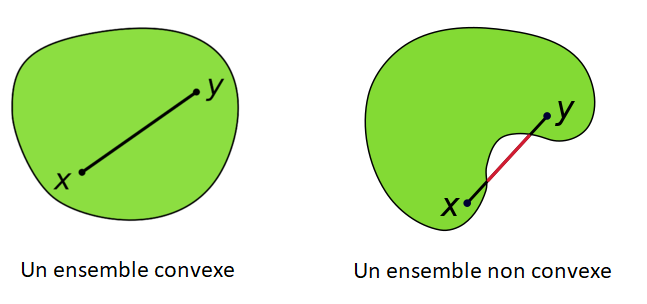
\includegraphics[scale=0.5]{figures/convexe1.png}
  \caption{Ensemble convexe}
  \label{}
\end{figure}



\begin{exemple}
  \begin{enumerate}
    \item Si $X$ est un espace vectoriel normé, $A = B(0, 1)$ et $x \in X$, on a $\frac{x}{\Vert x \Vert } \in B(0, 1)$. Alors $x \in \Vert x \Vert B(0, 1)$.
    \item Si $0 \in C$ convexe, alors $C$ est équilibré si et seulement si $C$ est balancé.
  \end{enumerate}
\end{exemple}


\begin{proof}
  On suppose que $C$ est balancé. Pour $x \in C \implies -x \in C$, donc $[-x, x] \in C$ par convexité.
\end{proof}

\begin{thm}\label{convexes-balances}
  Soit $X$ un espace vectoriel topologique. Les assertions suivantes sont équivalentes :

  \begin{enumerate}
    \item $X$ est un espace localement convexe (réel ou complexe);
    \item Il existe une base de voisinages de $0 \in X$ qui sont convexes, balancés (cerclés), absorbants.
  \end{enumerate}
\end{thm}

\marginpar{19-09-2023}

\begin{proof}
  \begin{enumerate}
    \item Si $X$ est un espace localement convexe, alors une base de voisinages de 0 est donnée par

    \[
    \mathcal{O} _{a, \varepsilon } = \{ x  \in X \mid \rho_a(x) \less \varepsilon  \}
    \]

    Les $\mathcal{O} _{a, \varepsilon }$ sont convexes, balancés et absorbants (TD).

    \item On utilise la jauge de Minkowski \ref{jauge_mink}.

    On pose \[
    \rho_C(x) = \mu_C(x).
    \]

    et on vérifie que $\rho_C$ est une semi-norme. Grâce au lemme \ref{lemme_mink}, on obtient les résultats suivants :

    \begin{enumerate}
      \item $\rho_C(x+y) \leq \rho_C(x)+ \rho_C(y)$, car $C$ est convexe ;
      \item $\rho_C(\lambda x) = \lambda \rho_C(x)$ si $\lambda \bg 0$ et $\rho_C(\lambda x) = \lvert \lambda  \rvert \rho_C(x)$, car $C$ est cerclé.

       %$\rho_C(\lambda x) = \rho_C((-\lambda )x)$ et on a

      %\[
      %\rho_C(\lambda x) = (-\lambda ) \rho_C(x) = \lvert \lambda  \rvert \rho_C(x),
      %\]

      %car $C$ est cerclé.

      $X$ muni de $\rho_C$ est un espace localement convexe.
    \end{enumerate}
  \end{enumerate}
\end{proof}

\begin{definition}[Jauge de Minkowski] \label{jauge_mink}
  Soit $X$ espace vectoriel réel ou complexe. On suppose que $C$ tel que $0 \in C$ est absorbant. Alors la jauge de Minkowski est définie comme suit :

  \[
  \mu_C(x) = \inf \{ \alpha \bg 0, x \in \alpha C \}.
  \]
\end{definition}

\begin{figure}[h!]
  \centering
  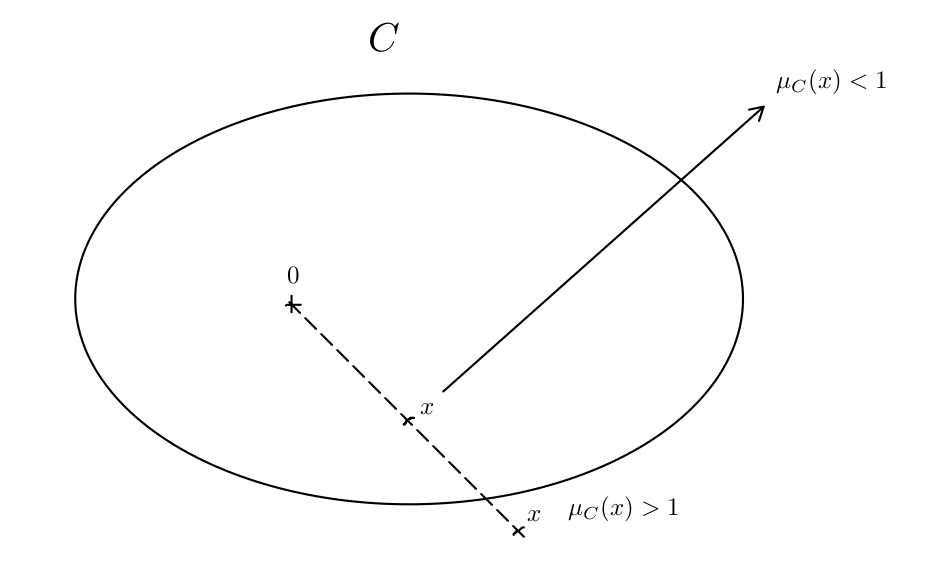
\includegraphics[scale=0.3]{figures/jaugem.png}
  \caption{La jauge de Minkowski}
  \label{}
\end{figure}

\begin{remark}
  Si $C$ est absorbant, alors $\forall x \in X$, $\mu_C(x) \less \infty$.
\end{remark}

\begin{lemma} \label{lemme_mink}
  Soit $C \subset X$ absorbant tel que $0 \in C$.
  \begin{enumerate}
    \item Si $\lambda  \geq 0$, $\mu_C(\lambda x)= \lambda \mu_C(x)$ ;
    \item Si $C$ est convexe, alors $\mu_C(x+y) \leq \mu_C(x)+ \mu_C(y)$ ;
    \item Si $C$ est cerclé, alors $\mu_C(\lambda x) = \lvert \lambda  \rvert \mu_C(x)$ ;
    \item $\{ x \in X, \mu_C(x) \less 1 \} \subset C \subset \{ x \in X, \mu_C(x) \leq 1 \} $.
  \end{enumerate}
\end{lemma}

\subsection{Théorème de Hahn-Banach}

Il y a la forme analytique et la forme géométrique de ce théorème.

\begin{thm}[De Hahn-Banach, forme analytique]
  Pour simplifier, on prend $X$ espace vectoriel sur $\mathbb{R}$. Soit $p : X \longrightarrow \mathbb{R}$ qui vérifie :
  \begin{itemize}
    \item [$\star$] $\forall x \in X, \forall \lambda \bg 0, p(\lambda x) = \lambda p(x)$ ;
    \item [$\star$] $\forall x, y \in X$, $p(x+y) \leq p(x) +p(y)$.
  \end{itemize}

  Soient $Y$ un sous espace vectoriel de $X$ et $l$ une forme linéaire sur $Y$ qui vérifie

  \[
  \forall x \in Y, l(x) \leq p(x), \forall x \in Y.
  \]

  Alors (prolongement) il existe $L$ forme linéaire sur $X$ telle que $L _{|Y} = l$ \textbf{et}

  \[
  \forall x \in X, L(x) \leq p(x).
  \]
\end{thm}

On l'applique aux espaces vectoriels normés, espaces localement convexes,...

\begin{thm}[Norme sur un espace dual] \label{norm-dual}
  Soit $X$ espace vectoriel normé, $X'$ formes linéaires continues sur $X$, $X'$ est un espace vectoriel normé. La norme sur $X'$ est définie de la façon suivante :

  \[
  \Vert L \Vert _{X'} \stackrel{\text{déf}}{=} \sup_{ \substack{x \in X \\ \Vert x \Vert =1 } } \lvert \langle L,x \rangle  \rvert = \sup_{ x \in X \setminus \{ 0 \} } \left\lvert \left\langle L, \frac{x}{\Vert x \Vert } \right\rangle  \right\rvert = \sup_{ x \in X \setminus \{ 0 \} } \frac{\lvert \langle L,x \rangle  \rvert}{\Vert x \Vert }.
  \]

\end{thm}


\begin{exo}
  Montrer que $\Vert \cdot \Vert _{X'} $ est une norme.
\end{exo}

Si $X$ est un espace vectoriel normé complet (de Banach), alors $X'$ l'est aussi.

\begin{corollary}[Prolongement isométrique de $l$ sur $Y$]
  Soit $X$ espace vectoriel normé, $Y \subset X$ sous espace vectoriel de $X$ et $l \in Y'$ avec

  \[
  \Vert l \Vert = \sup_{ \substack{\Vert y \Vert \leq 1 \\ y \in Y} } \lvert \langle l,y \rangle  \rvert.
  \]

  Alors il existe un prolongement $L$ de $l$ de même norme

  \[
  \sup_{ \substack{x \in X \\ \Vert x \Vert \leq 1 } }  \lvert \langle l,x \rangle  \rvert = \sup_{ \substack{y \in Y \\ \Vert y \Vert \leq 1 } } \lvert \langle l,y \rangle  \rvert.
  \]
\end{corollary}

\begin{proof}
  Par le théorème de Hahn-Banach, on pose $p$ telle que $p(x) = \Vert l \Vert _{Y'} \Vert x \Vert  $ (l'application définie ainsi vérifie les propriétés de $p$ nécessaires à l'application du théorème).

  Par Hahn-Banach, il existe $L$ une forme linéaire sur $X$ telle que
  \[
  L(x)  = \langle L,x \rangle \leq p(x) = \Vert l \Vert _{Y'} \Vert x \Vert.
  \]

  Mais
  \[
  \langle L, -x \rangle \leq \Vert l \Vert _{Y'} \Vert -x \Vert,
  \]

  donc
  \[
  \lvert \langle L,x \rangle  \rvert \leq \Vert l \Vert _{Y'} \Vert x \Vert.
  \]

  Ainsi, en divisant par $\Vert x \Vert $, on obtient le résultat suivant :

  \[
  \forall x \in X, \left\lvert \left\langle L, \frac{x}{\Vert x \Vert } \right\rangle  \right\rvert \leq \Vert l \Vert _{Y'}.
  \]

  Or si on prend $x \in Y$,

  \[
  \left\lvert \left\langle L, \frac{x}{\Vert x \Vert } \right\rangle  \right\rvert \leq \Vert l \Vert _{Y'} = \sup_{ y \in Y \setminus \{ 0 \} } \left\lvert \left\langle L, \frac{y}{\Vert y \Vert } \right\rangle  \right\rvert.
  \]

  Comme $Y \subset X$ (ce qui entraîne que $\sup_{ y \in Y \setminus \{ 0 \} } \left\lvert \left\langle L, \frac{y}{\Vert y \Vert } \right\rangle   \right\rvert \leq \sup_{ x \in X \setminus \{ 0 \} } \left\lvert \left\langle L, \frac{x}{\Vert x \Vert } \right\rangle   \right\rvert  $), on a donc égalité, d'où l'isométrie.
\end{proof}

\begin{corollary}
  $\forall x_0 \in X$ espace vectoriel réel, il existe $L_0 \in X', \Vert L_0 \Vert _{X'} = \Vert x_0 \Vert _{X} $.
\end{corollary}

\begin{proof}
  $Y = \mathbb{R} x_0$. Soit $l(tx_0) \stackrel{\text{déf}}{=} t \Vert x_0 \Vert ^2 $ forme linéaire continue sur $Y$.

  Alors, en posant $t=1$, on obtient

  \[
  \Vert l \Vert _{Y'} =  \Vert x_0 \Vert
  \]

  %\left( \sup_{ y \in Y \setminus \{ 0 \} } \frac{\lvert \langle L,y \rangle  \rvert}{ \Vert y \Vert } = \frac{\Vert x_0 \Vert ^2 }{\Vert x_0 \Vert } \right) =

  et, par le théorème de Hahn-Banach,

  \[
  \Vert L_0 \Vert _{X'} = \Vert x_0 \Vert _{X}.
  \]
\end{proof}

\begin{exo}
  Traduire Hahn-Banach dans le cas où $X$ est un espace localement convexe.
\end{exo}

\begin{thm}[De Hahn-Banach, forme géométrique]\label{hb-geo}
  Soit $X$ espace vectoriel normé (ou espace localement convexe). Soient $A, B \subset X$ convexes et disjoints.

  \begin{enumerate}
    \item On suppose que $A$ est ouvert. Alors il existe un hyperplan affine (d'équation $\langle L,x \rangle = \text{constante}$) $\mathscr{H} $ qui sépare au sens large $A$ et $B$.
    \item Si $A$ est fermé, $B$ est compact, alors il existe $\mathscr{H} $ hyperplan qui sépare $A$ et $B$ au sens strict.
  \end{enumerate}
\end{thm}

\begin{figure}[h!]
  \centering
  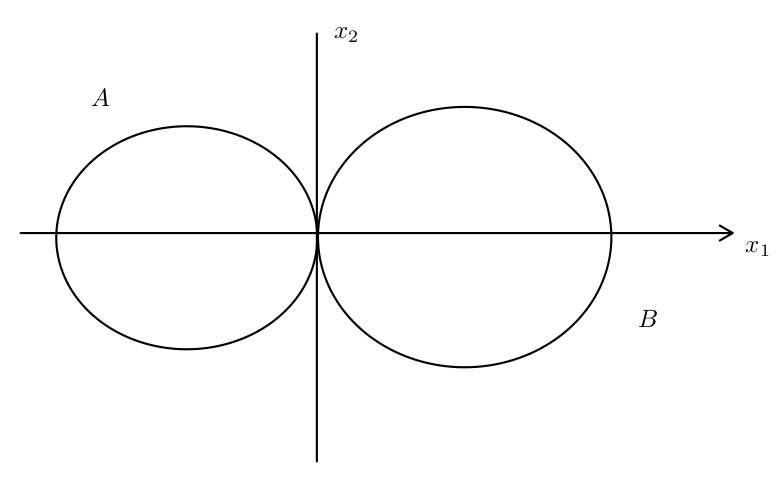
\includegraphics[scale=0.3]{figures/hb-geo.png}
  \caption{$A = \{ x_1 \less 0 \}, B = \{ x_2 \geq 0 \}, \mathscr{H} = \{ x_1 = 0 \}  $.}
  \label{}
\end{figure}

\section{Espaces localement convexes métrisables, espaces de Fréchet} \marginpar{26-09-2023}

\subsection{Topologies définies par une distance}

On rappelle la définition \ref{distance}.

\begin{definition}[Distances équivalentes]
  On dit que $d_1$ est équivalente à $d_2$ si et seulement si il existe \(C \bg 0\) tel que

  \[\frac{1}{C}d_1(x,y) \leq d_2(x,y) \leq C d_1(x,y).\]
\end{definition}

\(d_1 \sim d_2 \implies (X,d_1) \simeq (X,d_2)\), mais la réciproque est fausse.

\begin{exemple}
  On prend un espace métrique \((X,d)\) avec les distances

  \[\delta(x,y) = \frac{d(x,y)}{1+ d(x,y)} \text{ et } \delta'(x,y) = \inf(1, d(x,y)).\]

  Ces distances sont équivalentes entre elles.%, mais elles ne sont pas équivalentes à \(d\).
\end{exemple}

\begin{proof}

  \

  \begin{enumerate}
    \item Montrons que \((X, d) \sim (X, \delta')\). On remarque d'abord que

    \[\delta(x,y) = \frac{d(x,y)}{1+ d(x,y)} \leq d(x,y), \]

    ce qui veut dire que \((X, d) \prec (X, \delta)\) (car si \(\mathcal{O}\) est un ouvert pour \(\delta\), alors il le sera forcément pour \(d\)).

    Prenons
    \begin{equation}\label{bij-dist}
      f(t) = \frac{t}{1+t}.
    \end{equation}

    La fonction \(f\) est une bijection de \(\mathbb{R} ^{+}\) dans \([0, 1]\). En effet, montrons qu'il existe \(g : [0, 1] \to \mathbb{R} ^{+}\) telle que $g \circ f = f \circ g = \operatorname{id}$.

    On a

    \begin{gather*}
      \frac{t}{1+t} = s \implies t = ts+s \implies t = \frac{s}{1-s}.
    \end{gather*}

    Donc \(d(x,y) = \frac{\delta(x,y)}{1 - \delta(x,y)}\). Donc si \(d(x,y) \less \varepsilon\), alors \(d(x,y) \less \frac{\varepsilon}{1- \varepsilon}\). Donc \((X,\delta) \prec (X,d)\).

    \item Montrons que \(\delta \sim \delta'\).

    On a \[\delta = \frac{d}{1+d} \leq \begin{cases}
      1 \\
      \delta.
    \end{cases}\]

    En effet, cela vient du fait que \(\frac{d(x,y)}{1+d(x,y)} \underset{d(x,y) \to \infty }{\longrightarrow} 1\). Donc \[\delta(x,y) \leq \delta'(x,y).\]

    Mais \(\delta' \leq 2 \delta\). En effet, on distingue deux cas :

    \begin{enumerate}
      \item Si \(\delta \leq  1 \text{ et } \delta' = d, \text{ alors } d \leq 2 d \),
      \item Si \(\delta \geq  1 \text{ et } \delta' = 1, \text{ alors } 1 \leq 2 d \).
    \end{enumerate}

    \item Montrons que $\delta$ est une distance.

    \begin{enumerate}
      \item Montrons l'inégalité triangulaire. Si $d(x,y) \leq d(x,z) + d(z,y)$, montrons que $\delta(x,y) \leq \delta(x,z) + \delta(z,y)$.

      Est-ce que \(f(d(x,y)) \leq f(d(x,z))+ f(d(z,y))\), avec \(f\) définie dans \ref{bij-dist} ?

      \begin{enumerate}
        \item $f$ est croissante, donc \(f(d(x,y)) \leq f[d(x,z) + d(z,y)]\). Il suffit de voir que $f(t) \leq f(u)+f(v)$.

        \item Montrons la sous-additivité de $f$. Posons \[v  \mapsto \varphi(v) =  f(u+v) - f(u) - f(v). \]

        On a \(\varphi(0) = 0\), car \(f(0) =0\) et \(\varphi(v) = f'(u+v) - f'(v) \less 0\), car $f$ est une fonction croissante.
      \end{enumerate}
    \end{enumerate}
  \end{enumerate}
\end{proof}

\emph{Sous quelles conditions un espace localement convexe est métrisable ?}

On remarque par exemple que $\mathscr{F}([0, 1], \mathbb{R})$ muni de la topologie de la convergence simple n'est pas métrisable. Plus généralement, les topologies faibles ne sont pas métrisables, sauf si on travaille en dimension finie. Par ailleurs, \(X\) muni de la topologie grossière n'est pas métrisable (non séparée).

\begin{prop}\label{elc-metr}
  Soit \(X\) un espace localement convexe (donc séparé). Alors les assertions suivantes sont équivalentes.

  \begin{enumerate}
    \item \(X\) est métrisable.
    \item Il existe une base dénombrable de voisinages de 0 dans \(X\), et ce pour tout \(x \in X\).
    \item La topologie de \(X\) est engendrée par une famille dénombrable de semi-normes.
  \end{enumerate}
\end{prop}

\begin{proof}
  \begin{enumerate}
    \item \((1) \implies (2)\). La topologie sur \(X\) est équivalente à \((X,d)\). Soit \((X,d)\) un espace métrique. Il suffit de poser

    \[\mathcal{O} _{\frac{1}{n}} = \left\{ x \mid d(x,0) \less \frac{1}{n}\right\} \ (\mathbb{R} \text{ est archimédien}). \]

    Alors \(\forall \varepsilon \bg 0, \exists n \text{ tel que } \mathcal{O} _{\frac{1}{n}} \subset \mathcal{O} _{\varepsilon}\). Donc \(x + \mathcal{O} _{\frac{1}{n}}\) est une base dénombrable de voisinages de \(x\).

    \item \((2) \implies (3)\). On sait que \(\mathscr{T}\) topologie de \(X\) est donnée par une famille de semi-normes. Les voisinages de 0 dans \(X\) sont donnés par

    \[\mathcal{O} _{a, \varepsilon} = \bigcap _{i=1} ^{n} \mathcal{O} _{\varepsilon, a_i}, \text{ avec } i \in \{ 1, \dots, n \}.\]

    On rappelle que \(\mathcal{O} _{\varepsilon,a_i} = \{ x \mid \rho _{a_i} \less \varepsilon \}\).

    On peut choisir \(\varepsilon = \frac{1}{n}\). On sait qu'il existe une base dénombrable de voisinages de 0 dans \(X\). Soit \(U_n\) une base de voisinages dénombrable de 0. On pose

    \[\rho_n(x) = \mu _{U_n}(x).\]

    On prend les \(U_n\) convexes, balancés, absorbants comme dans le théorème \ref{convexes-balances} (c'est possible, car \(X\) est un espace localement convexe).

    \item \((3) \implies (1)\).

    \begin{enumerate}
      \item Soit \( (\rho_n)\) une famille dénombrable de semi-normes sur \(X\). On pose

      \[d(x,y) = \sum_{n=1}^{\infty} 2 ^{-n} \frac{\rho_n(x-y)}{1 + \rho_n(x-y)}.\]

      Montrons que \((X, \text{ELC}) \prec (X, d)\). Soit \(U \in \mathscr{T}\) (la topologie ELC). On se ramène aux voisinages de 0. On a

      \[U = \bigcap _{\text{finie}} \mathcal{O} _{\varepsilon, a}, a \in A. \]

      Comme il existe une base dénombrable de voisinages, on peut choisir

      \[U _{\varepsilon} = \bigcap _{j=1} ^{N} = \{ x \mid \rho _{j}(x-0)\less \varepsilon \}, \text{ avec } A= \mathbb{N}.\]

      Ce voisinage est inclus dans \(\left\{ x \mid \sum_{}^{} \rho_j(x-0) \leq N \varepsilon \right\}\).

      Montrons que \(U\) est un voisinage de \(x\) pour la topologie métrique \((X,d)\).

      Soit \(\varepsilon \bg 0\). On pose \(d(x,0) = \left( \sum_{1}^{N} + \sum_{N+1}^{\infty}\right) \frac{\rho_n}{1+ \rho_n}\). Or \(N\) est tel que

      \[\sum_{N+1}^{\infty} 2 ^{-n} \less \varepsilon \implies \sum_{N+1}^{\infty} 2 ^{-n} \frac{\rho_n}{1+ \rho_n} \less \varepsilon.\]

      De plus,

      \begin{gather}
        d(x,y) \leq \varepsilon + \sum_{n=1}^{N}  \frac{d_n}{1+d_n} \less \varepsilon + \sum_{n=1}^{N} d_n(x,y). \label{vois_un}
      \end{gather}

      Or \(\rho_n(x-y)\less \varepsilon\), car \(x \in y + U _{\varepsilon}\).

      Donc \ref{vois_un} devient

      \begin{gather*}
        d(x,y) \leq \varepsilon + N \varepsilon \text{ avec } N \text{ fixé.}
      \end{gather*}

      Donc \(\mathscr{T} \prec (X,d)\).

      \item Montrons que \((X,d) \prec \mathscr{T}\). On doit majorer \(\rho_m(x-y)\).

      Or \begin{gather*}
        d(x,y) = \sum_{n=1}^{\infty} 2 ^{-n} \frac{\rho_n(x-y)}{1+ \rho_n(x-y)} \geq 2 ^{-m} \frac{\rho_m(x-y)}{1 + \rho_m(x-y)}.
     \end{gather*}

     Et

     \begin{gather*}
       2 ^{m}d(x,y) \geq \frac{\rho_m(x-y)}{1 + \rho_m(x-y)} \geq  f(t).
     \end{gather*}

     Donc on a \(\rho_m(x,y) \leq  g(2 ^{m} d(x,y))\), où \(g\) est la réciproque de \(t \mapsto \frac{1}{1+t}\).
    \end{enumerate}
  \end{enumerate}
\end{proof}

\begin{prop}
  Soit \(X\) un espace localement convexe qui vérifie l'une des propriétés énoncées dans la proposition \ref{elc-metr} (i. e. métrisable). On note la topologie de \(X\) ELC par \(\mathscr{T}\). Alors \(X\) est complet pour \(\mathscr{T}\) si et seulement si \((X,d)\) est complet.
\end{prop}

\begin{proof}
  Cette proposition se démontre exactement comme \ref{elc-metr}.
\end{proof}

\begin{definition}
  Soit \(X\) un espace localement convexe. On dit que \(X\) est un \textbf{espace de Fréchet} si \(X\) est \textbf{métrisable et complet}.
\end{definition}

\begin{exemple}

  \

  \begin{enumerate}
    \item \emph{Les espaces localement convexes qui ne sont pas des Fréchet. }
    \begin{enumerate}
      \item \emph{Non métrisables.} \(\mathscr{F}([0, 1], \mathbb{R}) \) muni de la topologie de la convergence simple, les topologies faibles, \(\dots\)
    \end{enumerate}

    \item \emph{Les espaces localement convexes qui sont des Fréchet. } Les espaces de Banach, par exemple \(\mathscr{F}([0, 1], \mathbb{R}) \) muni de la topologie de la convergence uniforme, \(\mathcal{C}^{\infty}_0(K)\), \(\dots\)
  \end{enumerate}
\end{exemple}

\subsection{Espace de Schwarz \(\mathscr{S}(\mathbb{R} ^{d}) \subset \mathcal{C}^\infty(\mathbb{R}^d)\)}

\(\varphi \in \mathscr{S}(\mathbb{R}^d) \iff \rho _{\alpha, \beta}(\varphi) = \sup_{ \mathbb{R} } \left\lvert x ^{\alpha} D _{\varphi} ^{\beta} \right\rvert \less \infty\).

Montrons que \(\mathscr{S}(\mathbb{R})\) est complet. On va regarder \(\rho _{0, 0}, \rho _{0, 1}, \rho _{1, 0}, \rho _{1, 1}, \dots\)

\begin{enumerate}
  \item \(\rho _{0, 0}(\varphi _{p+q} - \varphi _{p}) \less \varepsilon\), donc \( \varphi _{p} \longrightarrow \varphi\), donc

  \[\sup_{ \mathbb{R} } \lvert \varphi _{p+q} (x) - \varphi _{p}(x) \rvert \less \varepsilon. \]

  En particulier pour tout \(K \subset \mathbb{R}\), \(\varphi_n\) est de Cauchy dans \(\mathcal{C}^0(K)\). Or \(\mathcal{C}^0(K)\) est complet, donc \(\varphi_n \underset{\text{uniformément}}{\longrightarrow} \varphi.\) Comme \(K\) est arbitraire, elle converge localement sur tout \(\mathbb{R}\). On a

  \[\rho _{0, 0}(\varphi _{p+q} - \varphi_p) \less \varepsilon, \]

  donc \[\rho _{0, 0}(\varphi - \varphi_p) \less \varepsilon.\]

  Donc \(\varphi _{p}\) converge pour \(\rho _{0,0}\).

  \item On a besoin de rappeler le lemme suivant :

  \begin{lemma}
    Si \(\varphi' \longrightarrow \psi\) uniformément et \(\varphi_n \longrightarrow \varphi\) simplement, alors \(\psi = \varphi'\).
  \end{lemma}
\end{enumerate}

\marginpar{10-10-2023}

\section{Topologie forte et topologie faible sur les espaces de Banach}

Soient \((E, \left\Vert \cdot \right\Vert) \) un espace de Banach (réel ou complexe) et \((E', \left\Vert \cdot \right\Vert')\) son dual topologique. On rappelle que

\[E' = \{ l \in \mathscr{L}(E, \mathbb{R}), \exists C \bg 0, \forall x \in E, \left\lvert \langle l,x \rangle  \right\rvert \leq C \left\Vert x \right\Vert^2 \}, \]

avec la norme sur le dual définie dans \ref{norm-dual}.

\((E', \left\Vert \cdot \right\Vert')\) est un espace de Banach, un cas particulier de \(\mathscr{L}(E,F)\), avec pour \(u \in \mathscr{L}(E,F)\),

\[\left\Vert u \right\Vert _{\mathscr{L}(E,F)} = \sup_{\substack {x \in E \\\left\Vert x \right\Vert_E \leq 1  }}  \left\Vert u(x) \right\Vert_F. \]

On affaiblit \((E,\left\Vert \cdot \right\Vert )\). Alors \(\sigma(E,E')\) est la topologie la moins fine qui rend continue toutes les formes linéaires sur \(E\). \(X \sim \sigma(E,E')\) est muni des semi-normes \(\left\lvert \langle l,x \rangle  \right\rvert = \rho_l(x)\). Un voisinage de 0 est défini de la manière suivante :

\[\mathcal{O} _{\underline{l}, \varepsilon} = \{ x \in E : \sup_{ 1 \leq  i \leq n} \langle l_i, x \rangle \less \varepsilon \}, \underline{l} = (l_1, \dots, l_n).\]

\subsection{Comparaison des topologies \((E, \left\Vert \cdot \right\Vert)\) et \(\sigma(E,E')\)}

\begin{lemma}
  Soit \(E\) un espace de Banach. Alors la norme définie

  \[x = \sup_{\substack {l \in E'\\ \left\Vert l \right\Vert' \leq 1 }} \left\lvert \langle l,x \rangle  \right\rvert = \langle l_0,x \rangle.  \]

  est telle que le \(\sup\) est atteint. On a \(\sup = \max\).
\end{lemma}

\begin{proof}
  On a \(x \neq 0\) par la définition de \(\left\Vert \cdot \right\Vert'\). Alors

  \[\left\lvert \left\langle l,\frac{x}{\left\Vert x \right\Vert } \right\rangle  \right\rvert \leq \left\Vert l \right\Vert' \leq 1.\]

  Alors \[\left\lvert \langle l,x \rangle  \right\rvert \leq  \left\Vert x \right\Vert \text{ pour tout } l \in E' \text{ tel que } \left\Vert l \right\Vert' \leq 1.\]

  Soit \(x_0\) et \(F\) tel que \(F = \mathbb{R} x_0\). Alors \(\forall \lambda \in \mathbb{R}, l_0(\lambda x_0) = \lambda\) et \(\left\Vert l_0 \right\Vert = \left\Vert x_0 \right\Vert.\) Par Hahn-Banach, on peut prolonger \(l_0\) en \(L_0\) sur tout l'espace de Banach.
\end{proof}

\begin{prop}
  \[(E,\left\Vert \cdot \right\Vert) \prec \sigma(E,E').\]

  Donc \(X \sim \sigma(E, E')\) est un espace localement convexe.
\end{prop}

\begin{proof}
  On a

  \[\rho_l(x) = \left\lvert \langle l,x \rangle  \right\rvert \leq \left\Vert l \right\Vert' \left\Vert x \right\Vert.  \]
\end{proof}

\begin{proof}[Autre démonstration]
  Montrons que \(\mathcal{O} _{\underline{l}, \varepsilon}\) est un ouvert de \((E, \left\Vert \cdot \right\Vert)\), i. e. \(\left\Vert x \right\Vert \less \delta\). On prend \(n\) formes linéaires \(l_i, i \in \{ 1, \dots, n \}\) et on considère

  \[ \left\Vert x \right\Vert = \sup_{ \left\Vert l \right\Vert' \leq 1  } \left\lvert \langle l,x \rangle  \right\rvert. \]

  Or \(\left\lvert \langle l_i,x \rangle  \right\rvert \less \varepsilon\) ... (à suivre).
\end{proof}

\begin{proof}
  Montrons que \(\sigma(E,E')\) est séparé. Soient \(x_1, x_2\) distincts. Montrons qu'il existe \(\mathcal{O}_1\) et \(\mathcal{O}_2\) de \(\sigma(E,E')\) tels que \(\mathcal{O}_1 \cap \mathcal{O}_2 = \emptyset\).

  Par le théorème de Hahn-Banach \ref{hb-geo}, pour \(A = \{ x_1 \}, B = \{ x_2 \} \) compacts et convexes, pour tout \((x,y) \in A \times B\), on a

  \[\langle l,x \rangle \less \alpha \less \langle l,y \rangle.\]

  Donc

  \[\langle l,x_1 \rangle \less \alpha \less \langle l,x_2 \rangle.\]

  On a \(x_1 \in \mathcal{O} _{\alpha,l}^{1} =\{ x : \langle l,x \rangle \less \alpha\}\) et \(\mathcal{O} _{\alpha,l} ^{2} = \{ y : \langle l,y \rangle \bg \alpha\}\), ces ouverts séparent \(x_1\) et \(x_2\).
\end{proof}


\begin{thm}
  \((E, \left\Vert \cdot \right\Vert )\) est strictement plus fine que \(\sigma(E, E')\) sauf en dimension finie.
\end{thm}

\begin{proof}
  On considère \(S = \{ \left\Vert x \right\Vert =1 \}\). Alors \(S = \overline{S}\), son adhérence.

  Soit \(x_0\) de norme plus petite que 1. Montrons que pour tout \(V\) voisinage de 0 dans \(\mathscr{T}\), \(V \cap S \neq \emptyset\). On a

  \[V = \{ x : \left\lvert \langle l_i,x - x_0 \rangle  \right\rvert \less \varepsilon, 1 \leq i \leq n \}.\]

  Comme \(\operatorname{dim}(E) = \infty\), il existe \(y_0 \neq 0\) tel que \(\langle l_i, y_0 \rangle =0, \forall i\). On a

  \begin{gather*}
    g(t) = \left\Vert x_0 + t y_0 \right\Vert.
  \end{gather*}

  On a \(g(0) = \left\Vert x_0 \right\Vert \less 1\) et \(g(\infty) = +\infty\). La fonction \(g\) est continue, donc il existe \(t_0 \in (0, \infty)\) tel que \(\left\Vert x_0 + t_0 y_0 \right\Vert = 1\). Donc \(x_0 + t_0 y_0 \in S\) et \(x_0 + t_0 y_0 \in V\), car

  \[\left\lvert \langle l_i, (x_0 + t_0 y_0) - x_0 \rangle  \right\rvert = \left\lvert \langle l_i, t_0 y_0 \rangle  \right\rvert = \left\lvert t_0 \langle l_i, y_0 \rangle  \right\rvert = 0 \less \varepsilon.\]
\end{proof}

\begin{remark}
  \(\forall t \in \mathbb{R}, \langle l_i, x_0 + t y_0 \rangle = 0\). Alors \(V\) contient toute une droite.
\end{remark}

\begin{remark}
  Pour \(E\) Banach séparable, \(B_E\) boule unité fermée de \((E,\left\Vert \cdot \right\Vert)\) est métrisable pour \(\sigma(E,E')\).

  Si \(E\) est réfléxif (c'est-à-dire que l'injection naturelle dans son bidual est surjective), alors \(B_E = \{ \left\Vert x \right\Vert \leq 1 \} \) est un espace métrique compact pour \(\mathcal{O}(E, E')\).
\end{remark}

\subsection{Théorème de Banach-Steinhaus, suites faiblement et fortement convergentes}

\begin{thm}
  Soient \(E,F\) espaces de Banach et \((T_a) _{a \in A} \in \mathscr{L}(E,F)\) telle que

  \[\forall x \in E, \sup_{ a \in A } \left\Vert T_a x \right\Vert _{F} \less + \infty.\]

  Alors \[\sup_{ a \in A } \left\Vert T_a \right\Vert \less +\infty \text{ (bornée en norme),}\]

  i. e. \(\exists C \bg 0, \forall x \in E, \forall \alpha \in A, \left\Vert T_\alpha(x)\right\Vert \leq C \left\Vert x \right\Vert\).
\end{thm}


\begin{corollary}
  Soit \(T_n \in \mathscr{L}(E,F)\) avec \(\left\Vert T_n \right\Vert \less +\infty\) avec \(\forall x \in E, T_n x \underset{n \to \infty}{\longrightarrow}y \in F\). On note \(y = Tx\). Alors \(T \in \mathscr{L}(E,F)\) et \(T = \lim \inf  T_n\).
\end{corollary}

\begin{proof}
  Montrons que \(T_n\) est linéaire. En effet,

  \begin{gather*}
    T_n(\lambda x + \lambda' x') = \lambda T_n(x)+ \lambda'T_n(x').
  \end{gather*}

  Par passage à la limite, on obtient \(T(\lambda x+ \lambda' x') = \lambda T(x) + \lambda' T(x')\).

  Montrons l'autre partie du corollaire. Par Banach-Steinhaus, si on considère \(A = \mathbb{N}\), pour tout \(x \in E\), \(T_n x\) est convergente, donc bornée, i. e. \(\left\Vert T_n x \right\Vert \less \infty\), donc \(\displaystyle\sup_{ n } T_n \less C\) comme \(\left\Vert T_n x \right\Vert \leq \left\Vert T_n \right\Vert \left\Vert x \right\Vert\).

  Par passage à la limite, on obtient \(\left\Vert T x \right\Vert \leq C \left\Vert x \right\Vert\), avec \(C = \lim \inf \left\Vert T_n \right\Vert\).
\end{proof}

\begin{definition}
  Soit \(E\) espace de Banach. \(B \subset E\) est bornée si et seulement si \[\exists C \geq 0, \forall x \in B, \left\Vert x \right\Vert \leq C. \]
\end{definition}

\begin{corollary}
  \(B \subset E\) est bornée si et seulement si \(\forall l \in E', l(B) \subset \mathbb{R}\) est borné.
\end{corollary}

\subsubsection{Suites faiblement et fortement convergentes}

\begin{definition}[Suite fortement convergente]
  Soit \(x_n \text{ une suite de }  E\). On dit que \(x_n\) est fortement convergente lorsque \(x_n \longrightarrow x \iff \left\Vert x_n -x \right\Vert \longrightarrow 0\).
\end{definition}

\begin{definition}[Suite fortement convergente]
  Soit \(x_n \text{ une suite de }  E \). On dit que \(x_n\) est faiblement convergente lorsque \(x_n \longrightarrow x \iff \forall l \in E', \langle l,x_n \rangle \longrightarrow \langle l,x \rangle\).

  On note alors \(x_n \stackrel{\text{w}}{\longrightarrow} x\) (avec \emph{weak} qui signifie faible en anglais) ou \(x_n \rightharpoonup x\).
\end{definition}


\begin{corollary}

  \

  \begin{enumerate}
    \item Si \(x_n \longrightarrow x\) dans \((E, \left\Vert \cdot \right\Vert)\), alors \(x_n \longrightarrow x\) dans \(\sigma(E,E')\).
    \item Si \(x_n \longrightarrow x\), alors \(x_n\) est bornée dans \(E\) et \(\left\Vert x \right\Vert_E \leq \lim \inf \left\Vert x_n \right\Vert\).
    \item Si \(x_n \longrightarrow x\) et \(l_n \longrightarrow l\), alors \(\langle l_n,x_n \rangle \longrightarrow \langle l,x \rangle\).
  \end{enumerate}
\end{corollary}

\begin{proof}
  \begin{enumerate}
    \item Soit \(l \in E'\). Alors

    \[\left\lvert \langle l,x_n - x \rangle  \right\rvert \leq \left\Vert l \right\Vert' \left\Vert x_n -x \right\Vert  \underset{n \to \infty}{\longrightarrow} 0.\]

    \item \(T_n : E \longrightarrow \mathbb{R}\). Alors on définit

    \[T_n l = \langle l, x_n \rangle \longrightarrow \langle l,x \rangle =  T l,  \]

    car \(x_n\) tend faiblement vers \(x\). Alors d'après le corollaire, \(\sup \left\Vert T_n \right\Vert \less \infty\), avec \(T \in (E')' = E''\) et \(\left\Vert T \right\Vert'' \leq \lim \inf \left\Vert x_n \right\Vert\), donc \(\left\lvert T l \right\rvert = \left\lvert \langle l,x \rangle  \right\rvert \) par passage à la limite.

    \item \[\langle l_n,x_n \rangle - \langle l,x \rangle = \langle l, x_n - x \rangle + \langle l, x_n - x \rangle.\]

    Or \(\langle l, x_n - x \rangle \longrightarrow 0\), car \(x_n \longrightarrow x\) et \(\langle l, x_n - x \rangle \longrightarrow 0\), car \(\left\lvert \langle l_n -l, x_n \rangle  \right\rvert \leq  \left\Vert l_n - l \right\Vert \left\Vert x_n \right\Vert \longrightarrow 0 \).
  \end{enumerate}
\end{proof}

\end{document}
